\documentclass[10pt]{sigplanconf}

\usepackage{amsmath}
\usepackage{amsthm}
\usepackage{float}
\usepackage{pifont}
\usepackage{graphicx}
\usepackage{multirow}
\usepackage{fancyvrb}
\usepackage{url}
\usepackage{verbatim}
\usepackage{alltt}

\newtheorem{definition}{Definition}

\newcommand{\kvd}[1]{\textbf{\sffamily #1}}
\newcommand{\ident}[1]{\textnormal{\sffamily #1}}
\newcommand{\fqt}{\`{}\hspace{-0.25em}\`{}}

\newcommand{\val}[1]{\texttt{#1}}

\begin{document}

\toappear{Unpublished draft.}
\title{Type providers}
%\subtitle{\large Well-typed programs only go wrong when the schema changes.\\~}

\authorinfo
  {Authors}
  {Affliations}
  {emails@domain}

\maketitle

\begin{abstract}
~
 
What is the problem?

~

Why is it important?

~

What do we do?

~

What follows from that?

~
\end{abstract}

\section{Introduction}
Modern applications do not run in vacuum. They execute in \emph{information rich} environments,
access data from relational databases, external files and from increasingly important web-based 
services. Stable, organized \emph{information spaces} are now available via the web \cite{providers-techreport}.

Despite this, few strongly-typed programming languages and tools are able to seamlessly integrate 
external information sources as if they were strongly-typed components from a programmer's 
perspective. 

The recent version of F\# introduced a \emph{type provider} mechanism \cite{providers-techreport} 
which makes it possible to view diverse external data sources as statically typed components. However,
this mechanism rises a number of concerns. Most importantly, if the type of the component depends on
a schema of external data source, the type safety of program is relativized with respect to possible
schema change of the data source.

~

TODO

\newpage

\begin{itemize}
\item Give a unified model of \emph{information spaces} using RDF triples and sketch how different 
  data sources (including relational databases, XML and WorldBank) can be mapped to the triple model. 
  We then distinguish between \emph{schema} and \emph{data} in the \emph{information space}.

\item We describe \emph{type-bridging mechanism} -- a formal model of F\# 3.0 type providers --
  that specifies how to map an information space into a programming language. The mechanism takes
  some information from the \emph{information space} as the \emph{schema} and based on the schema,
  maps the information space into types and values. The choice of schema is reflected in the 
  provided types.

\item We formalize the notion of \emph{relativized type safety} -- informally, a type safe program 
  using our type-bridging mechanism does not go wrong as long as the \emph{schema} in the 
  information space does not change. 

\end{itemize}

\newpage

\section{F\# type providers}
F\# type providers \cite{providers-techreport} provide a bridging mechanism that exposes external
data sources as statically typed components. Technically, type providers are compile-time components
that provide the \emph{signature} (a static type) of the external component together with its 
\emph{implementation} (code that obtains data and exposes it in a format matching the signature).

The following example uses the Freebase \cite{providers-freebase} type provider to print a list of
computer scientists:
%
\begin{equation*}
\begin{array}{l}
\kvd{\#r}~\texttt{"DataStore.Freebase.dll"}\\[0.5em]
\kvd{let}~\ident{data}=\ident{DataStore.Freebase}()\\
\kvd{for}~\ident{c}~\kvd{in}~\ident{data.Science.\fqt Computer Scientists\fqt}~\kvd{do}\\
\quad\ident{printf}~\texttt{"\%s"}~\ident{c.Name}
\end{array}
\end{equation*}
%
The type provider is referenced on the first line. It provides a type \ident{DataStore.Freebase} that
is constructed on the first line. The provided type has a property \ident{Science} which returns an
instance of another type with a property \ident{\fqt Computer Scientists\fqt}. The property has a type
\ident{ComputerScientistsEntity~list} where \ident{ComputerScientistsEntity} is another provided type
with property \ident{Name} (among many others).

The provider also provides an implementation of the types and properties. Using a type erasure mechanism
(similar to the one used in Java Generics \cite{types-java-erasure}), the \ident{ComputerScientistsEntity}
type is erased to a general \ident{FreebaseEntity} type and the access to \ident{Name} property is
erased to a call \ident{c.GetStringValue(\texttt{"Name"})}.

\subsection{Questions}
The example rises a number of questions -- many of them are already answered in the F\# type 
providers technical report \cite{providers-techreport}. In this paper, we focus on the following two
themes.

\paragraph{Representation.} To implement a type provider (e.g. for the Freebase data source), the 
developer needs to write F\# code that connects to a data source and generates types based on the
information available.

This mechanism is powerful, but it is difficult to analyse formally, because a type provider may 
execute arbitrary code. Thus our first aim is to find a simpler model that is more amenable to 
formal analysis (and might be also used to simplify the implementation of certain type providers).

\paragraph{Type safety.} The above code is only correct as long as the Freebase schema does not change in 
certain ways. For example, renaming \ident{Name} property to \ident{\fqt Full name\fqt} would break
the above code, because the \ident{Name} is reflected at the type-level (and 
\ident{c.GetStringValue(\texttt{"Name"})} would fail because the value for the key
\texttt{"Name"} is not available).

On the other hand, changing the name of ``Tomas Petricek'' to ``Tom\'a\v{s} Pet\v{r}\'i\v{c}ek'' is 
not a problem, because the change is only made in part of information that is available at value 
level. After such change, the code will print different results, but it will still work.

Thus our second aim is to analyse the type provider and specify what schema changes are safe
and which are not. A type provider is type-safe with respect to a schema change if the schema
change does not break the provided types and the provided implementation.

\section{Information spaces}
The F\# type provider mechanism makes a reasonable assumption that there is no single universal
schema language for describing \emph{information spaces} -- and thus it allows arbitrary F\# code
in the type provider.

However, to model type providers formally, we need to find a model of \emph{information space} that 
is simple and amenable to formal analysis, but powerful enough to model a wide range of data
sources accessible using type providers including hierarchical data (i.e.\ XML files), SQL databases, 
multi-dimensional data (such as Freebase, the World Bank data set) etc. 

\subsection{The RDF data model}
Our formal model of information spaces is based on the Resource Description Framework (RDF), which 
\emph{``is a language for representing information about resources in the World Wide Web''} \cite{semweb-rdf}.
RDF is based on the idea of modelling information using a graph. The nodes of the graph represent
resources (identified using an URI) or primitive values and the nodes represent properties.

\begin{figure}
\begin{center}
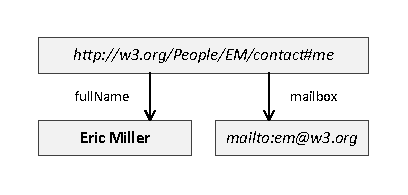
\includegraphics[scale=1]{figs/rdf.pdf}
\end{center}
\vspace{-1.5em}
\caption{Graph representation of data}
\label{fig:rdf-example}
\end{figure}

Figure~\ref{fig:rdf-example} shows a basic example adapted from \cite{semweb-rdf}. It shows a model
with three edges and two nodes. One edge represents a primitive value (a string) and two 
other edges represent URIs (unique identifier of a person and email). The nodes associate values
with the root edge and annotate them as \ident{fullName} and \ident{mailbox}. 
% The same dataset can be also stored using the following XML/RDF \cite{semweb-rdf-xml} notation:
%
% {\footnotesize \begin{verbatim}
% <rdf:RDF xmlns:rdf="http://w3.org/...rdf-syntax-ns#"  
%          xmlns:contact="http://w3.org/.../contact#">
%   <contact:Person 
%       rdf:about="http://w3.org/People/EM/contact#me">
%     <contact:fullName>Eric Miller</contact:fullName>
%     <contact:mailbox rdf:resource="mailto:em@w3.org"/>
%     <contact:personalTitle>Dr.</contact:personalTitle> 
%   </contact:Person>
% </rdf:RDF>
% \end{verbatim}
% }

The RDF model can be presented in form of \emph{triples} consisting of \emph{subject},
\emph{predicate} and \emph{object} (where subject and object are nodes and predicate
is an edge in the graph). For the purpose of this paper and our model of type providers, 
we use a simplified formal model based on triples:

\newcommand{\iprim}{\mathcal{P}}
\newcommand{\calv}{\mathcal{V}}
\newcommand{\calr}{\mathcal{R}}

\begin{definition}
Given a set of primitive values $\iprim$, a set of entity identifiers $?$ and a
set of relation identifiers $?$

an \emph{information space} $(\calv, \calr)$ is a triple of values $\calv$ and relations between
pairs of values $\calr \in \calv \times \calv$. The relations are undirected, meaning that 
$(v_1, v_2) \in \calr \Leftrightarrow (v_2, v_1) \in \calr$. 
\end{definition}

\subsection{Examples} 
The previous simple definition is general enough to model a number of real-world data sources.
We look at three examples showing how databases, XML and multi-dimensional data sets 
can be viewed as information spaces.

\paragraph{DB}

\paragraph{XML}



\newpage
~
\newpage

\bibliographystyle{abbrvnat}
\bibliography{providers}

\end{document}
